%%%%%%%%%%%%%%%%%%%%%%%%%%%%%%%%%%%%%%%%%%%%%%%%%%%%%%%%%%%%%%%%%%%
%                                                                 %
%                 Packages / Grundeinstellungen                   %
%                                                                 %
%%%%%%%%%%%%%%%%%%%%%%%%%%%%%%%%%%%%%%%%%%%%%%%%%%%%%%%%%%%%%%%%%%%


% Festlegung des Allgemeinen Dokumentenformat
\documentclass[a4paper,12pt,parskip=half,headsepline,DIV=12,numbers=noenddot]{scrartcl}

%%%%%% Muss in die documentclass %%%%%%%%
%BCOR12mm, Korrektur fuer die Bindung
%DIV12 DIV-Wert fuer die Erstellung des Satzspiegels
%numbers=noenddot

% Keine floats in andere Sections
\usepackage[section]{placeins}

% Weitere Pakete
\usepackage{microtype}
\usepackage{scrhack}
\usepackage{caption}
\usepackage{fontspec}
\usepackage{csquotes}
\usepackage{pdflscape}
\usepackage{float}

% Booktabs Tabellen
\usepackage{booktabs}
\usepackage{tabularx}

% Grafiken aus PNG Dateien einbinden
\usepackage{graphicx}

% Deutsche Sonderzeichen und Silbentrennung nutzen
\usepackage[ngerman]{babel}
\usepackage{blindtext}

% Eurozeichen einbinden
\usepackage[right]{eurosym}

% Kopf- und Fußzeilen
\usepackage[headsepline,autooneside=false]{scrlayer-scrpage}
\clearpairofpagestyles

% Schriftart 
\usepackage{lmodern}

% Floatende Bilder ermöglichen
\usepackage{floatflt}

% Für Tabellen
\usepackage{array}

% tikz
\usepackage{tikz}
\usetikzlibrary{calc,arrows,math}
\usetikzlibrary{shapes.geometric,positioning}

%% Schaltpläne nach europäischen Richtlinien
\usepackage[european]{circuitikz}
\tikzset{x=1mm,y=1mm}

\usepackage{siunitx}
\sisetup{output-decimal-marker={,},detect-all}

% Mehrseitige Tabellen ermöglichen
\usepackage{longtable}

% Unterstützung für Schriftarten
%\newfontfamily\popp{Poppins}
%\fontspec{Poppins}
%\setkomafont{disposition}{\fontspec{Poppins}}

% Paket für Boxen im Text
\usepackage{fancybox}

% Bricht lange URLs "schön" um
\usepackage[hyphens,obeyspaces,spaces]{url}

% Paket für Textfarben
\usepackage{color}

% Mathematische Symbole importieren
\usepackage{amssymb}

% Erzeugt Inhaltsverzeichnis mit Querverweisen zu den Abschnitten (PDF Version)
\usepackage[bookmarksnumbered,hyperfootnotes=false]{hyperref}
\hypersetup{
     colorlinks=true,
     linkcolor=black,
     filecolor=blue,
     citecolor = black,      
     urlcolor=blue,
}

% Zitierung nach IEEE
%\usepackage[
%backend=biber,
%style=ieee,
%autocite=inline,
%]{biblatex}
%\addbibresource{bibtex/hauptdatei.bib}

% Zitierung nach APA

\usepackage[
backend=biber,
style=apa,
autocite=inline,
]{biblatex}
\addbibresource{bibtex/hauptdatei.bib}


% Paket für Zeilenabstand
\usepackage{setspace}

% Für Bildbezeichner
\usepackage{capt-of}

% Für Stichwortverzeichnis
\usepackage{makeidx}

% Konfiguriere das Inhaltsverzeichnis
\usepackage{tocbasic}
\DeclareTOCStyleEntries[
  raggedentrytext,
  %numwidth=0pt, if numbers=noenddot is not set
  numsep=1ex,
  dynnumwidth,
]{tocline}{chapter,section}
\DeclareTOCStyleEntries[
  linefill=\TOCLineLeaderFill,
]{tocline}{section,subsection,subsubsection,paragraph,subparagraph}

% Für Listings
\usepackage{listings}
\lstset{numbers=left, numberstyle=\tiny, numbersep=5pt, keywordstyle=\color{black}\bfseries, stringstyle=\ttfamily,showstringspaces=false,basicstyle=\footnotesize,captionpos=b, breaklines=true}

% Indexerstellung
\makeindex

% Abkürzungsverzeichnis
\usepackage[printonlyused, smaller, withpage]{acronym}

% Schriftart Helvetica verwenden
%\usepackage{helvet}
%\renewcommand\familydefault{\sfdefault}

\hypersetup{pdfinfo={
Title={Titel der Arbeit},
Author={Ruben Allenstein}
}}

%%%%%%%%%%%%%%%%%%%%%%%%%%%%%%%%%%%%%%%%%%%%%%%%%%%%%%%%%%%%%%%%%%%
%                                                                 %                    
%                     Beginn des Inhalts                          %
%                                                                 %
%%%%%%%%%%%%%%%%%%%%%%%%%%%%%%%%%%%%%%%%%%%%%%%%%%%%%%%%%%%%%%%%%%%

%%%%%%%%%%%%%%%%%%%%%%%%%%%%%%%%%%%%%%%%%%%%%%%%%%%%%%%%%%%%%%%%%%%
%  Special Characters:                                            %
%                                                                 %
%             \& \% \$ \# \_ \{ \}                                %
%             \textasciitilde (~)                                 %
%             \textasciicircum (^)                                %     
%             \textbackslash (\)                                  %                    
%      \glqq Text\grqq{} für Anführungszeichen                    %
%%%%%%%%%%%%%%%%%%%%%%%%%%%%%%%%%%%%%%%%%%%%%%%%%%%%%%%%%%%%%%%%%%%

\begin{document}

% Definition Header Sections sollen in der Kopfzeile stehen Kopfzeile mit Unterstrich
\automark[subsection]{section}
\KOMAoptions{headsepline=true}
%\ihead{Kopfzeile innen}
%\chead{Kopfzeile außen}
\ohead{\headmark}

% Definition footer \pagemark steht für Seitennummer
%\ifoot{Fußzeile innen}
%\cfoot{Fußzeile Mitte}
\ofoot{\pagemark}

% Hier werden die Trennvorschläge inkludiert
%%%%%%%%%%%%%%%%%%%%%%%%%%%%%%%%%%%%%%%%%%%%%%%%%%%%%%%%%%%%%%%%%%%%%%%%%%%%%%%%%%%%%%%%%%%
%    Hier müssen alle Wörter eingetragen werden, welche Latex von nicht korrekt trennt    %
%                bzw. bei denen man die genaue Trennung vorgeben möchte.                  %
%%%%%%%%%%%%%%%%%%%%%%%%%%%%%%%%%%%%%%%%%%%%%%%%%%%%%%%%%%%%%%%%%%%%%%%%%%%%%%%%%%%%%%%%%%%

\hyphenation{
Film-pro-du-zen-ten
Lux-em-burg
Soft-ware-bau-steins
zeit-in-ten-siv
}


% Leere Seite am Anfang
%\thispagestyle{empty} % erzeugt Seite ohne Kopf- / Fusszeile
%\mbox{}
%\newpage

% Titelseite %
%%%%%%%%%%%%%%%%%%%%%%%%%%%%%%%%%
%           Deckblatt           %
%%%%%%%%%%%%%%%%%%%%%%%%%%%%%%%%%

\thispagestyle{empty}
\begin{figure}[h!]
 \centering
 
\includegraphics[width=0.6\textwidth]{src/abbildungen/logo.png}
\end{figure}
\begin{center}
\large\textbf{Fachbereich II \\ Management und Informationssysteme}\\
\large\textbf{Wirtschaftsinformatik B.Sc.}\\
\vspace{1cm}
%%%%%%%%%%%%%%%%%%%%%%%%%%%%%Für Hausarbeit%%%%%%%%%%%%%%%%%%%%%%%%%%%%%%%%%%%
%\large\textbf{Modul\\ Modulname}\\
%%%%%%%%%%%%%%%%%%%%%%%%%%%%%%%%%%%%%%%%%%%%%%%%%%%%%%%%%%%%%%%%%%%%%%%%%%%%%%
%%%%%%%%%%%%%%%%%%%%%%%%%%%Für Bachelorarbeit%%%%%%%%%%%%%%%%%%%%%%%%%%%%%%%%%
\LARGE\textbf{Bachelorarbeit}\\
\large{zur Erlangung des akademischen Grades \\ Bachelor of Science}\\
%%%%%%%%%%%%%%%%%%%%%%%%%%%%%%%%%%%%%%%%%%%%%%%%%%%%%%%%%%%%%%%%%%%%%%%%%%%%%%
\vspace*{\fill}
\line(1,0){450}\\
\doublespacing
\textbf{\Large{Titel}}\\
\textbf{\large{Untertitel}}\\
\line(1,0){450}\\
\end{center}
\vspace*{\fill}
\onehalfspacing
\begin{flushleft}
\begin{tabular}{llll}
  \textbf{Vorgelegt von:} & & Maxi Mustermensch MatNr. 00000 \\
%  & & Second Author MatNr. 00000 \\
%  & & Third Author MatNr. 00000 \\
\textbf{Vorgelegt am:} & & \today &\\
%%%%%%%%%%%%%%%%%%%%%%%%%%%%%Für Hausarbeit%%%%%%%%%%%%%%%%%%%%%%%%%%%%%%%%%%%
%\textbf{Dozent:in:} & & Prof. Dr. Maxi Mustermensch & \\
%%%%%%%%%%%%%%%%%%%%%%%%%%%%%%%%%%%%%%%%%%%%%%%%%%%%%%%%%%%%%%%%%%%%%%%%%%%%%%
%%%%%%%%%%%%%%%%%%%%%%%%%%%Für Bachelorarbeit%%%%%%%%%%%%%%%%%%%%%%%%%%%%%%%%%
\textbf{Erstgutachter:in:} & & Prof. Dr. Maxi Mustermann & \\
\textbf{Zweitgutachter:in:} & & Prof. Dr. Maxi Musterfrau &\\
%%%%%%%%%%%%%%%%%%%%%%%%%%%%%%%%%%%%%%%%%%%%%%%%%%%%%%%%%%%%%%%%%%%%%%%%%%%%%%
\end{tabular}
\end{flushleft}

\newpage

% Singlespacing (Default)
\singlespacing

% Abstract falls gewünscht
%\onehalfspacing
%\thispagestyle{empty}
%\input{abstract}
%\newpage

% Seitenzählung nach dem Inhaltsverzeichnis bei 1 beginnen
%\setcounter{page}{1}

% Inhaltsverzeichnis anzeigen
\thispagestyle{empty}
\tableofcontents
\newpage

% Header für den Inhalt 
\KOMAoptions{headsepline=true}
\ohead{\headmark}

% Input Inhalt
\section{Einleitung}\label{einleitung}
\Blindtext
% Beispiel für Bildintegration
\FloatBarrier
\begin{figure}[!ht]
 \centering
 
\includegraphics[width=0.8\textwidth]{src/abbildungen/logo.png}
  \caption[Beschreibung]{Beschreibung~\autocite[S.14]{mf2005}}
\label{fig:Beschreibung}
\end{figure}
\FloatBarrier
\Blindtext


\section{Hauptabschnitt Zwei}\label{hauptabschnitt}

\Blindtext
\Blindtext

\subsection{Unterabschnitt von Zwei}\label{unterabschnitt_1}

\Blindtext
\Blindtext
\Blindtext
% Beispiel: Tabelle 
\begin{table}[!ht]
  \centering
    \caption[Beispieltabelle]{Beispieltabelle~\autocite[S.400]{KnutThea2009}}
    \label{table:Beispieltabelle}
    \begin{tabular}{ | l | c | }
      \hline
      Überschrift 1 & Überschrift 2 \\ \hline 
      Info 1 & Info 2 \\ \hline
      Info 3 & Info 4 \\ \hline
      \hline
      \multicolumn{2}{|c|}{Info in einer Zelle} \\
      \hline
    \end{tabular}
  \end{table}
\Blindtext


Lorem ipsum dolor sit amet, consetetur \ac{eu} sadipscing elitr, sed diam nonumy eirmod tempor invidunt ut labore et dolore magna aliquyam erat, sed diam voluptua. At vero eos et accusam et justo duo dolores et ea rebum. Stet clita 
kasd gubergren, no sea takimata sanctus est Lorem ipsum dolor sit amet. \ac{eu} Lorem ipsum dolor sit amet, consetetur sadipscing elitr, sed diam nonumy eirmod tempor invidunt ut labore et dolore magna aliquyam erat, sed diam voluptua. 
At vero eos et accusam et justo duo dolores et ea rebum. Stet clita kasd gubergren, no sea takimata \ac{https} sanctus est Lorem ipsum dolor sit amet.

\subsection{Neuer Unterabschnitt von Zwei}\label{unterabschnitt_2}

\Blindtext
  \begin{table}[!ht]
    \centering
    \caption[Beispieltabelle 2]{Beispieltabelle 2}
    \label{table:Beispieltabelle_2}
  \begin{tabular}{ccc}\toprule
    A&B&C \\ \midrule
    a&b&c \\ \cmidrule{1-3}
    1&2&3\\ \bottomrule
    \end{tabular}
  \end{table}
\Blindtext
\Blindtext



  
\subsection{Neuer Unterabschnitt von Zwei}\label{unterabschnitt_3}

\begin{quote}
  \singlespacing \small
  "`Lorem ipsum dolor sit amet, consectetur adipiscing elit, sed do eiusmod tempor incididunt ut labore et dolore magna aliqua. Et odio pellentesque diam volutpat commodo sed. Donec pretium vulputate sapien nec 
  sagittis aliquam. Nullam ac tortor vitae purus faucibus."'~\autocite[S. 189]{KnutThea2009}
\end{quote}

\Blindtext

\subsubsection{Unterabschnitt von Unterabschnitt von Zwei}\label{unterunterabschnitt}
\Blindtext

\begin{figure}
 \centering
\begin{circuitikz}
  \draw (0,80) node[vcc]    (vcc) {+ \SI{5}{\volt}};
  \draw (0,60) node (d) {};
  \draw (0,30) node (r3) {};
  \draw (0,15) node (r4) {};
  \draw (0,0)  node[rground] (gnd) {};
  \draw (vcc) to[leDo] (d.center);
  \draw (d.center)  to[R=$R_3$,a={\SI{1}{\kilo\ohm}}]  (r3.center);
  \draw (r3.center)  to[R=$R_4$,a={\SI{1}{\kilo\ohm}}]  (r4.center);
  \draw (r4.center)  to  (gnd);
\end{circuitikz}
  \caption[Schaltung]{Schaltung}
  \label{fig:Schaltung}
\end{figure}

\Blindtext
% Beispiel für Formeln
Die Zuordnung aller möglichen Werte, welche eine Zufallsvariable annehmen kann nennt man \emph{Verteilungsfunktion} von $X$.

\begin{quote}
Die Funktion F: $\mathbb{R} \rightarrow$ [0,1] mit $F(t) = P (X \le t)$ heißt Verteilungsfunktion von $X$. vgl.~\autocite[S.55]{mf2005}
\end{quote}

\begin{quote}
Für eine stetige Zufallsvariable $X: \Omega \rightarrow \mathbb{R}$ heißt eine integrierbare, nichtnegative reelle Funktion 
$w: \mathbb{R} \rightarrow \mathbb{R}$ mit $F(x) = P(X \le x) = \int_{-\infty}^{x} w(t)dt$ die \emph{Dichte} oder \emph{Wahrscheinlichkeitsdichte} 
der Zufallsvariablen $X$. vgl.~\autocite[S.225-323]{KnutThea2009}
\end{quote}

\Blindtext

\subsubsection{Neuer Unterabschnitt von Unterabschnitt von Zwei}\label{neuerunterunterabschnitt}

\Blindtext

\section{Hauptabschnitt Drei}\label{hauptabschnitt3}
\Blindtext

% beispiel für quellcode listings
\lstset{language=xml}
\begin{lstlisting}[float=ht!, frame=htrbl, caption={die datei {\normalfont \ttfamily  data-config.xml} dient als beispiel für xml quellcode}, label={lst:dataconfigxml}]
<dataconfig>
  <datasource type="jdbcdatasource" 
              driver="com.mysql.jdbc.driver"
              url="jdbc:mysql://localhost/bms_db"
              user="root" 
              password=""/>
  <document>
    <entity name="id"
        query="select id, htmlbody, sentdate, sentfrom, subject, textbody
        from mail">
    <field column="id" name="id"/>
    <field column="htmlbody" name="text"/>
    <field column="sentdate" name="sentdate"/>
    <field column="sentfrom" name="sentfrom"/>
    <field column="subject"  name="subject"/>
    <field column="textbody" name="text"/>
    </entity>
  </document>
</dataconfig>
\end{lstlisting}
\Blindtext

\subsection{Unterabschnitt von Drei}\label{hauptabschnitt3.1}

\Blindtext

\lstset{language=java}
\begin{lstlisting}[float=ht!, frame=htrbl, caption={das listing zeigt java quellcode}, label={lst:result2}]
import java.io.*;
import javax.servlet.*;
import javax.servlet.http.*;

public class HelloServlet extends HttpServlet {

  protected void doGet(HttpServletRequest  request, 
      HttpServletResponse response)
      throws IOException, ServletException {

      response.setContentType("text/html");
      PrintWriter out = response.getWriter();
      out.println("<!doctype html><html>");
      out.println("<head> <meta charset='utf-8'>");
      out.println("<title>webapp</title> </head>");
      out.println("<body>Hello</body>");
      out.println("</html>");
      ServletContext context = getServletContext();
      context.log("simple logging");
  }
}
\end{lstlisting}
\Blindtext

\begin{enumerate}
\item Eine Aufzählung
  \begin{itemize}
  \item mit Unterpunkten
  \end{itemize}
\item Ein weiterer Punkt
  \begin{itemize}
  \item mit zusätzlichen Stichpunkten
  \item wertvolle Information
  \end{itemize}
\end{enumerate}

\subsection{Neuer Unterabschnitt von Drei}\label{hauptabschnitt3.2}

\Blindtext

\section{Fazit}\label{fazit}

\Blindtext
\Blindtext

\newpage

% Literaturverzeichnis anzeigen
\ohead{Literaturverzeichnis} % Korrektur für Header 
\phantomsection
\addcontentsline{toc}{section}{Literaturverzeichnis}
\renewcommand\refname{Literaturverzeichnis}
\printbibliography
\newpage

% Abbildungsverzeichnis anzeigen
\ohead{\headmark}
\listoffigures
\newpage
\addcontentsline{toc}{section}{Abbildungsverzeichnis}

% Tabellenverzeichnis anzeigen
\listoftables
\newpage
\addcontentsline{toc}{section}{Tabellenverzeichnis}

% Listingverzeichnis anzeigen
\renewcommand{\lstlistlistingname}{Listingverzeichnis}
\lstlistoflistings
\newpage
\addcontentsline{toc}{section}{Listingverzeichnis}

% Abkürzungsverzeichnis anzeigen
\ohead{Abkürzungsverzeichnis} % Korrektur für Header 
\section*{Abkürzungsverzeichnis}\label{Abkuerzungsverzeichnis}
%%%%%%%%%%%%%%%%%%%%%%%%%%%%%%%%%%%%%%%%%%%%%%%%%%%%%%%%%%%%%%%%%%%%%%%%%%%%%%%%%%%%%%%%%
%                             Mit Einrückung im Verzeichnis                             %                     
%  Alle Abkürzungen müssen mit: \acro{acronym}[shortname]{fullname} eingetragen werden. %
%                         Im Fließtext mit \ac{acronym} aufrufen.                       %
%                 Erster Aufruf: fullname (shortname), danach shortname.                %                                   
%%%%%%%%%%%%%%%%%%%%%%%%%%%%%%%%%%%%%%%%%%%%%%%%%%%%%%%%%%%%%%%%%%%%%%%%%%%%%%%%%%%%%%%%%

\begin{addmargin}[1.5em]{0em}

    \begin{acronym}[HTTPS] %längster shortname muss eingetragen werden.
    
        \acro{eugh}[EuGH]{Europäischer Gerichtshof}
    
        \acro{eu}[EU]{Europäische Union}

        \acro{https}[HTTPS]{Hypertext Transfer Protocol Secure}
    
    \end{acronym}

\end{addmargin}
\newpage
\addcontentsline{toc}{section}{Abkürzungsverzeichnis}

% Kein Header für Anhang (Deckblatt) 
\KOMAoptions{headsepline=false}
\ohead{}

% Beginn Anhang
%%%%%%%%%%%%%%%%%%%%%%%%%%%%%%%%%
%      Deckblatt Anhang         %
%%%%%%%%%%%%%%%%%%%%%%%%%%%%%%%%%

\phantomsection
\addcontentsline{toc}{section}{Anhang}
\vspace*{\fill}
\begin{center}
    \doublespacing
    \line(1,0){450}\\
    \textbf{\Huge{Anhang}}\\
    \line(1,0){450}
    \singlespacing
    \begin{verbatim}
      
    \end{verbatim}
    \end{center} 
\vspace*{\fill}
\newpage

% Anhang römisch 
\renewcommand{\thesection}{\Roman{section}} 
\renewcommand{\thesubsection}{\Roman{subsection}}
\setcounter{section}{0}

% Header Anhang (Inhalt)
\KOMAoptions{headsepline=true}
\ohead{\headmark}
\automark{subsection}

% Input Anhang 
\subsection{Anhang Eins}
\Blindtext
% Beispiel für Bildintegration
\begin{figure}[!ht]
    \centering
    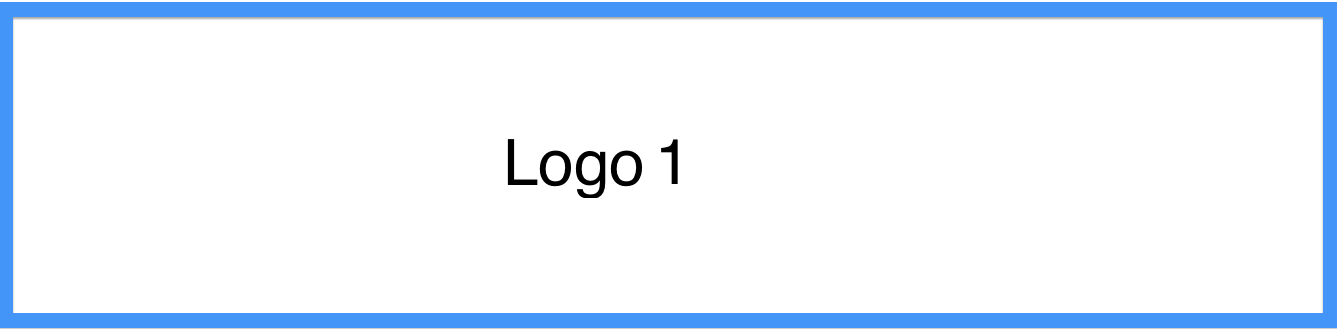
\includegraphics[width=0.3\textwidth,angle=0]{src/anhang/abbildungen/abb_anhang1.png}
    \caption[Abbildung im Anhang]{Abbildung im Anhang}
   \label{fig:Abbildung im Anhang}
   \end{figure}

\Blindtext

\subsection{Anhang zwei}
\Blindtext

\newpage

% Selbstständigkeits Erklärung
\phantomsection
\addcontentsline{toc}{section}{Selbstständigkeitserklärung}

% Header für Erklärung
\ohead{Selbstständigkeitserklärung}

% Input Erklärung
\section*{Selbstständigkeitserklärung}

\vspace{1cm}
Ich versichere, die von mir vorgelegte Arbeit selbstständig verfasst zu haben. Alle Stellen, die wörtlich oder sinngemäß aus veröffentlichten oder nicht veröffentlichten Arbeiten anderer entnommen sind, 
habe ich als entnommen kenntlich gemacht. Sämtliche Quellen und Hilfsmittel, die ich für die Arbeit benutzt habe, sind angegeben. Die Arbeit hat mit gleichem Inhalt bzw. in wesentlichen 
Teilen noch keiner anderen Prüfungsbehörde vorgelegen.



\begin{displaymath}
\begin{array}{ll}
Unterschrift:~~~~~~~~~~~~~~~~~~~~~~~~~~~~~~~~~~~~~~~~~~
& Ort, Datum:~~~~~~~~~~~~~~~~~~~~~~~~~~~~~~~~~~~~~~~~~~
\end{array}
\end{displaymath}


% Leere Abschlussseite
%\newpage
%\thispagestyle{empty} % erzeugt Seite ohne Kopf- / Fusszeile
%\mbox{}

\end{document}
